\documentclass[10pt,a4paper]{article}
\usepackage[margin=2.2cm]{geometry}
\usepackage{amsmath,amssymb,bm}
\usepackage{graphicx}
\usepackage{booktabs}
\usepackage{tabularx}
\usepackage{tikz}
\usetikzlibrary{arrows.meta,calc}
\usepackage[numbers,sort&compress]{natbib}
\usepackage{microtype}
\usepackage{listings}
\usepackage{xcolor}
\usepackage[hidelinks]{hyperref}
\usepackage{cleveref}

\newcommand{\un}[1]{\,\mathrm{#1}}
\definecolor{codebg}{HTML}{F6F5F1}
\definecolor{kw}{HTML}{1F5FBF}
\definecolor{cm}{HTML}{5F7F5F}
\lstset{language=C++, basicstyle=\ttfamily\small, keywordstyle=\color{kw}\bfseries,
  commentstyle=\color{cm}\itshape, backgroundcolor=\color{codebg}, frame=single, rulecolor=\color{codebg},
  columns=fullflexible, keepspaces=true, showstringspaces=false, xleftmargin=4pt, xrightmargin=4pt,
  morekeywords={Image,Detection}}

\title{The Vision Library\\[2pt]\large Ball Balancing Platform --- student guide}
\author{Ball Balancing Platform project}
\date{Library version 1.0 --- \today}

\begin{document}
\maketitle

\begin{abstract}
This guide covers everything you can use in \texttt{tracking.cpp}: the camera image you receive,
what the ball looks like in it and why, the conventions for reporting where you found the ball,
and how fast your code has to be to keep up on the FireBeetle. It then walks through the starter
tracker and the standard techniques for making it more accurate and more robust
\citep{gonzalez2018digital,szeliski2022computer}.
\end{abstract}

\tableofcontents

%======================================================================
\section{Your job}
%======================================================================
\begin{lstlisting}
void track(const Image& image, Detection& ball);
\end{lstlisting}
The library calls \texttt{track()} once for every camera frame, 30 times a second by default.
Find the ball and report its centre \textbf{in pixels}:
\begin{lstlisting}
ball.found = true;
ball.x = 163.4f;   // column
ball.y = 118.9f;   // row
\end{lstlisting}
If you cannot find it, set \texttt{ball.found = false}. Do not guess. The library then converts
your pixel position to millimetres on the plate, accounting for the lens and for refraction
through the plate, and hands it to \texttt{control()}. You never deal with millimetres here.

%======================================================================
\section{The image}
%======================================================================
\begin{center}
\begin{tabularx}{\textwidth}{>{\ttfamily}lX}
\toprule
image.width(), image.height() & $320\times240$ pixels (QVGA).\\
image.gray(x, y) & Brightness $0$--$255$.\\
image.red(x, y), green, blue & Colour channels, $0$--$255$ each.\\
\bottomrule
\end{tabularx}
\end{center}
\begin{itemize}
  \item Pixel $(0,0)$ is the \textbf{top-left} corner; $x$ grows to the right and $y$ grows down.
        Pixel $(i,j)$ covers the square $[i,i+1)\times[j,j+1)$, so its centre is at
        $(i+0.5,\,j+0.5)$. Report the ball centre in the same continuous coordinates, which is why
        the starter code adds $0.5$.
  \item The camera delivers \textbf{RGB565}: 5 bits of red, 6 of green and 5 of blue. Each channel
        is scaled back to $0$--$255$, but only has 32 (red, blue) or 64 (green) distinct levels.
        Smooth gradients therefore show bands (\cref{fig:frames}, right).
  \item \texttt{gray()} is the standard luma, computed in integers:
        $Y=(77R+150G+29B+128)/256$ (ITU-R BT.601 weights).
  \item Reading outside the image is undefined and can crash your program. Keep $0\le x<$
        \texttt{width()} and $0\le y<$ \texttt{height()}.
\end{itemize}

%======================================================================
\section{What the camera sees}
%======================================================================
The camera sits $134\un{mm}$ below the plate's top surface, at its centre, looking \emph{up}
through the transparent acrylic plate. So in the image:
\begin{itemize}
  \item The \textbf{ceiling} is the bright background. It is slightly brighter on one side
        (a window), and darker towards the corners because of lens vignetting.
  \item The \textbf{plate} is a large disc, very slightly darker than its surroundings
        ($\approx8\%$ of the light is reflected at its surfaces).
  \item The three \textbf{joint bosses} under the plate are small dark blobs, about $100\un{px}$
        from the centre, at the leg positions. They are the classic false detection.
  \item The \textbf{ball} is seen from below. A steel ball looks dark, because it reflects the dark
        base, with a brighter rim. With the default lighting a white ball's underside is also
        dark; switch on the ring light (Simulated hardware) to light it up. A $20\un{mm}$ ball is
        about $22\un{px}$ across.
\end{itemize}

\begin{figure}[h]
\centering
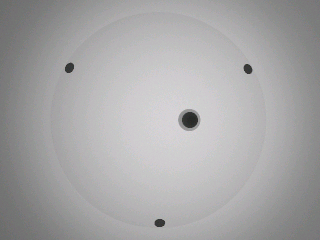
\includegraphics[width=0.48\textwidth]{../physics/figures/frame_noisy.png}\hfill
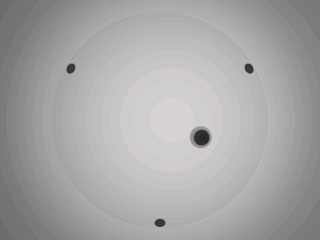
\includegraphics[width=0.48\textwidth]{../physics/figures/frame_clean.png}
\caption{Simulated camera frames. Left: a normal frame, with noise. Right: noise switched off
(Simulated hardware, image noise $=0$), which shows the RGB565 banding of the vignetted
ceiling.}
\label{fig:frames}
\end{figure}

\subsection{Image and plate directions}
With the plate level, the image centre $(160,120)$ looks at the plate centre. Moving the ball
towards plate $+x$ moves it \textbf{right} in the image, and towards plate $+y$ moves it
\textbf{down} (\cref{fig:axes}). Because the camera looks from below, the image is a mirror image
of what you see standing over the platform. You only report pixels, so this does not affect your
code. It does matter when you compare the camera view with the 3D view.

\begin{figure}[h]
\centering
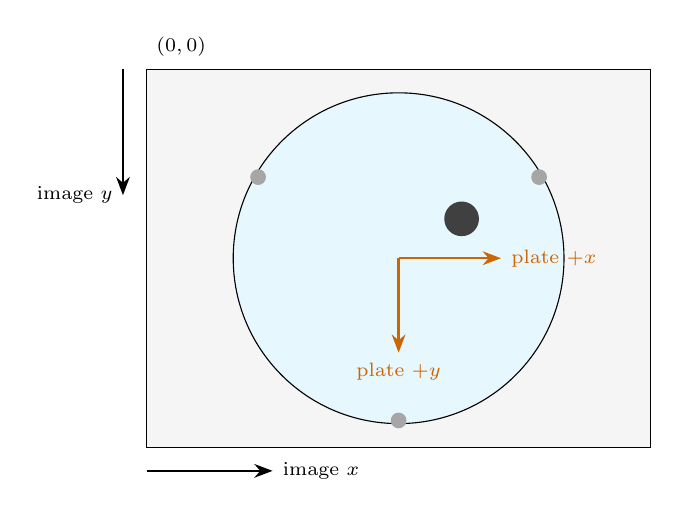
\begin{tikzpicture}[scale=0.02,>=Stealth]
  \draw[fill=gray!8] (0,0) rectangle (320,-240);
  \node[font=\scriptsize, anchor=south west] at (0,2) {$(0,0)$};
  \draw[->, thick] (0,-255) -- (80,-255) node[right, font=\scriptsize] {image $x$};
  \draw[->, thick] (-15,0) -- (-15,-80) node[left, font=\scriptsize] {image $y$};
  \draw[fill=cyan!10] (160,-120) circle (105);
  \foreach \a in {-150,-30,90} \fill[gray!70] ({160+103*cos(\a)},{-120-103*sin(\a)}) circle (5);
  \draw[->, orange!80!black, thick] (160,-120) -- (225,-120) node[right, font=\scriptsize] {plate $+x$};
  \draw[->, orange!80!black, thick] (160,-120) -- (160,-180) node[below, font=\scriptsize] {plate $+y$};
  \fill[black!75] (200,-95) circle (11);
\end{tikzpicture}
\caption{The camera image with the plate's axes overlaid. Plate $+y$ points \emph{down} in the
image, because the camera looks up from below.}
\label{fig:axes}
\end{figure}

\subsection{Scale and distortion}
At the centre of the image one pixel is about $0.9\un{mm}$ at the height of the ball's centre.
The wide-angle lens has barrel distortion, which squeezes the edges: there, one pixel covers more
millimetres. The library corrects for this, and for the $\approx1\un{mm}$ sideways shift that the
$5\un{mm}$ acrylic plate causes near its edge. Your job is only to find the right pixel.

\subsection{Imperfections you will meet}
\begin{itemize}
  \item \textbf{Noise}: every pixel fluctuates by a few grey levels from frame to frame (photon
        shot noise and read noise).
  \item \textbf{Motion blur}: the exposure lasts $6\un{ms}$. A ball moving at $200\un{mm/s}$
        moves $1.2\un{mm}$, more than a pixel, during it.
  \item \textbf{Rolling shutter}: the rows are captured one after another over $15\un{ms}$, so a
        fast ball is slightly skewed.
  \item \textbf{Perspective}: the camera sees a sphere's silhouette, whose centre is not exactly
        the projection of the ball's centre. Near the plate edge the difference is about
        $1\un{mm}$.
\end{itemize}
You can change the noise, the exposure, the lens and the lighting in the simulator to see how
your tracker copes.

%======================================================================
\section{The starter tracker}
%======================================================================
\begin{lstlisting}
void track(const Image& image, Detection& ball) {
    const int threshold = 80;        // pixels darker than this belong to the ball
    const float searchRadius = 90;   // ignore the dark joint bosses near the plate edge
    const float cx = image.width() / 2.0f, cy = image.height() / 2.0f;
    long sumX = 0, sumY = 0, count = 0;
    for (int y = 0; y < image.height(); y++)
        for (int x = 0; x < image.width(); x++) {
            const float dx = x - cx, dy = y - cy;
            if (dx * dx + dy * dy > searchRadius * searchRadius) continue;
            if (image.gray(x, y) < threshold) { sumX += x; sumY += y; count++; }
        }
    if (count < 20) { ball.found = false; return; }
    ball.found = true;
    ball.x = float(sumX) / count + 0.5f;
    ball.y = float(sumY) / count + 0.5f;
}
\end{lstlisting}
It \emph{thresholds} the image (dark pixels are ball) and takes the \emph{centroid} of the
selected pixels:
\begin{equation}
  \bar x=\frac{1}{N}\sum_{(x,y)\in S}x+\tfrac12,\qquad \bar y=\frac{1}{N}\sum_{(x,y)\in S}y+\tfrac12 .
\end{equation}
It works, but it has weaknesses you can fix:
\begin{enumerate}
  \item The circular mask that hides the bosses also hides the ball when it is near the plate
        edge.
  \item The fixed threshold breaks when the lighting, exposure or ball changes.
  \item Every pixel is visited every frame, which is slow on the FireBeetle.
  \item A binary centroid ignores partly covered edge pixels, so it is less precise than it could
        be.
\end{enumerate}

%======================================================================
\section{Techniques}
%======================================================================
\paragraph{Weighted centroid.} Weigh each pixel by how much darker it is than the background,
$w=\max(0,\,B-Y)$, and compute $\bar x=\sum wx/\sum w$. Edge pixels then contribute in proportion
to how much of the ball they contain, which gives sub-pixel accuracy.

\paragraph{Adaptive threshold.} Choose the threshold from the image itself. One way is the
midpoint between the typical background and ball brightness. Another is Otsu's method, which
picks the threshold that best separates the histogram into two classes \citep{otsu1979threshold}.

\paragraph{Search window (tracking).} The ball moves at most a few pixels between frames. Search
only a window, say $50\times50$ pixels, around the last position, and fall back to the whole
image when you lose it. This is about $30\times$ less work, and the bosses are excluded
automatically unless the ball is right next to one.

\paragraph{Connected components.} Group neighbouring dark pixels into blobs and keep the one that
looks like the ball: the right area ($\approx380\un{px}$ for $20\un{mm}$), round, and close to
where it was. This rejects bosses and other dark specks wherever the ball is
\citep{gonzalez2018digital}.

\paragraph{Background subtraction.} Store an image of the empty plate (or a slowly updated
average), then look for pixels that differ from it. This works for any ball colour and removes
the vignetting and the window gradient.

\paragraph{Circle fitting.} Find edge pixels and fit a circle to them, or vote for circle centres
with a Hough transform \citep{duda1972use}. This is more robust when the ball is partly
occluded, but much more expensive.

\paragraph{Sanity checks.} Reject a detection whose area is far from the expected size, or that
jumped implausibly far, and report \texttt{found = false} instead. A missing measurement is
better than a wrong one: \texttt{control()} sees \texttt{ball.found} and can hold still.

%======================================================================
\section{Speed: the FireBeetle budget}
%======================================================================
On the real platform your code runs on the FireBeetle's ESP32-S3 at $240\un{MHz}$, many times
slower than a PC. The simulator measures how long your \texttt{track()} and \texttt{control()}
take on the PC, multiplies by the slowdown factor in Setup, and delays the result by that much.
The Simulation tab shows both numbers.
\begin{itemize}
  \item At $30\un{fps}$ there are $33\un{ms}$ per frame. Time spent in your code is delay in the
        control loop, so less is better (see the control library guide).
  \item A full scan visits $76\,800$ pixels. Each \texttt{gray()} call converts RGB565 to luma.
        Scan a window, or every second pixel for a coarse search, instead.
  \item Use \texttt{float} and \texttt{int}, never \texttt{double}. The ESP32-S3 has no hardware
        for \texttt{double}.
  \item Avoid allocating memory (\texttt{new}, \texttt{std::vector} growth) inside
        \texttt{track()}.
\end{itemize}

%======================================================================
\section{Checking your tracker}
%======================================================================
The simulator knows exactly where the ball is. In the Simulation tab:
\begin{itemize}
  \item The camera view draws your detection as a green cross on the frame your code received.
  \item The \emph{ball x} and \emph{ball y} plots show the true position (line) and your
        measurement (dots). The gap between them is your tracking error, after the library's
        conversion to millimetres.
  \item \texttt{log("name", value)} plots anything else, for example your blob area or the
        threshold you chose.
\end{itemize}

\section{Things to try}
\begin{enumerate}
  \item Replace the binary centroid with a weighted centroid. Compare the measurement noise in the
        plots with the image noise set to $2$.
  \item Add a search window around the last position, and compare the FireBeetle time shown in
        the Simulation tab.
  \item Make the tracker work for the white ball with the ring light on, without changing the
        threshold by hand.
  \item Remove the circular mask and reject the bosses with a blob-size check instead. Can you
        now track the ball all the way to the plate edge?
\end{enumerate}

\bibliographystyle{plainnat}
\bibliography{references}

\end{document}
